\begin{figure}[htpb]
	\centering\capstart{}
	\subfloat[Initial Noisy Data \newline
		\(\snr{x} = \SI{4.11}{\dB}\)]
	{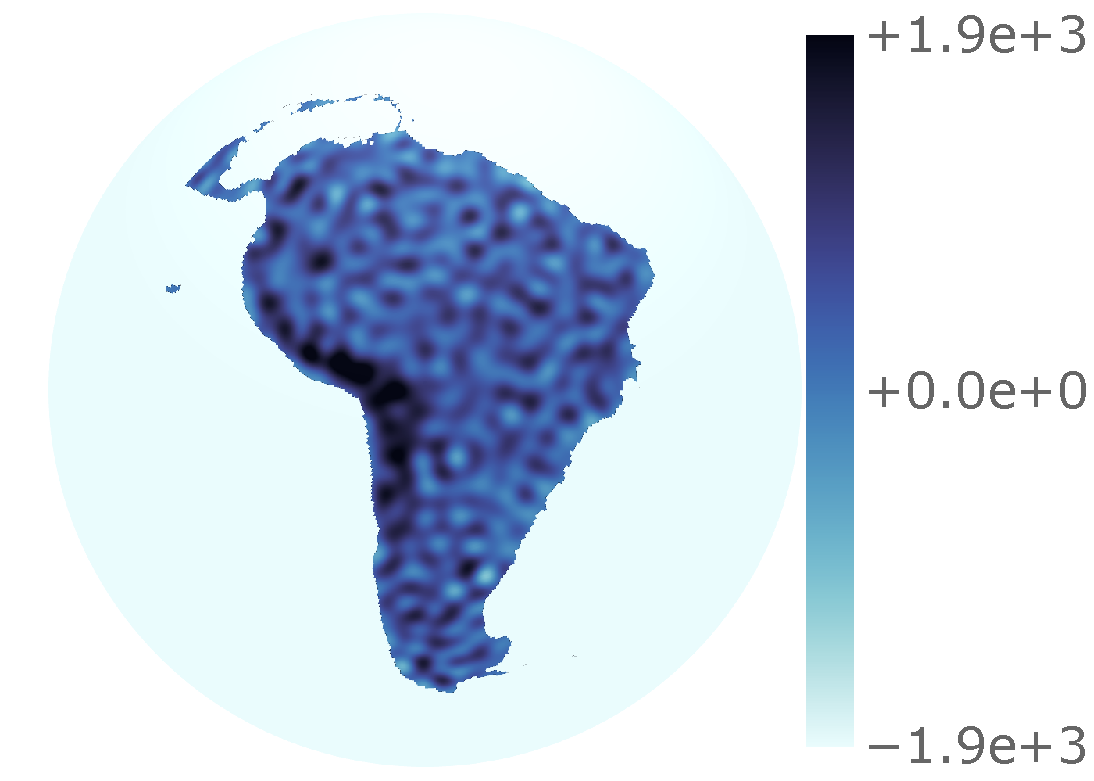
\includegraphics[trim={4 7 3 6},clip,width=.5\textwidth]{slepian_south_america_-10noise_2smoothed_L128_res512_real.pdf}}
	\hfill
	\subfloat[Denoised \(N_{\sigma}=2\) \newline
		\(\snr{d} = \SI{5.67}{\dB}\)]
	{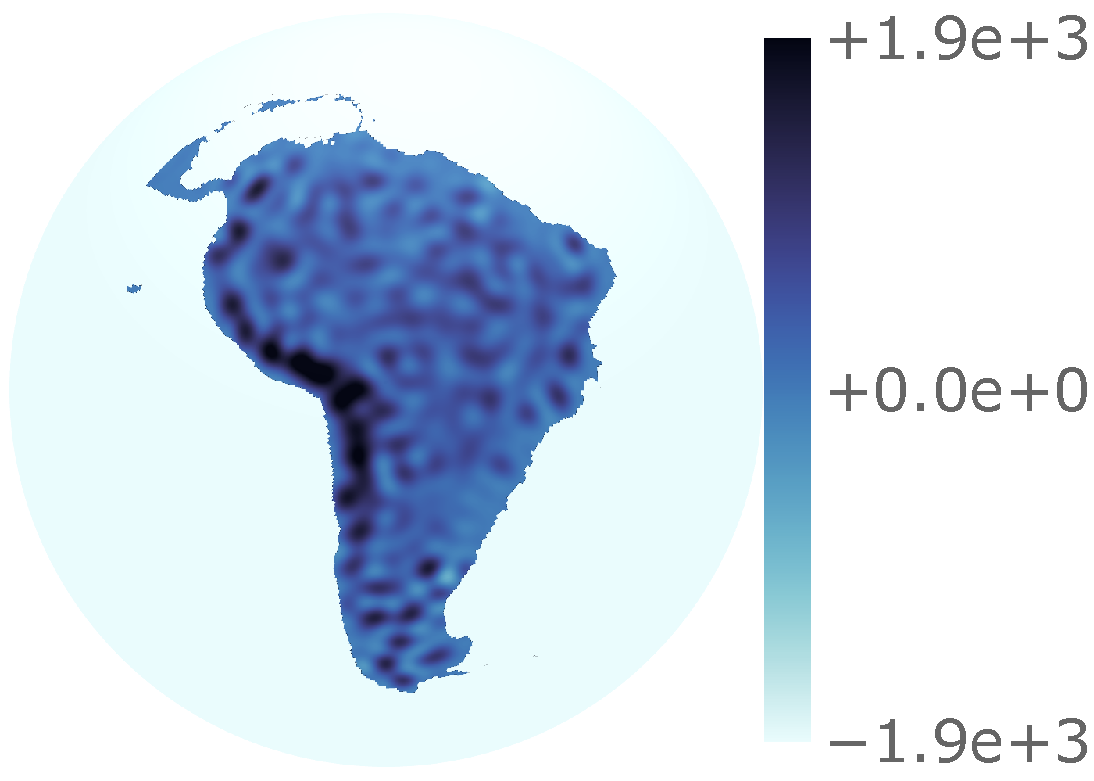
\includegraphics[trim={4 7 3 6},clip,width=.5\textwidth]{slepian_south_america_2smoothed_L128_-10snr_2n_denoised_res512_real.pdf}}
	\newline
	\subfloat[Denoised \(N_{\sigma}=3\) \newline
		\(\snr{d} = \SI{4.60}{\dB}\)]
	{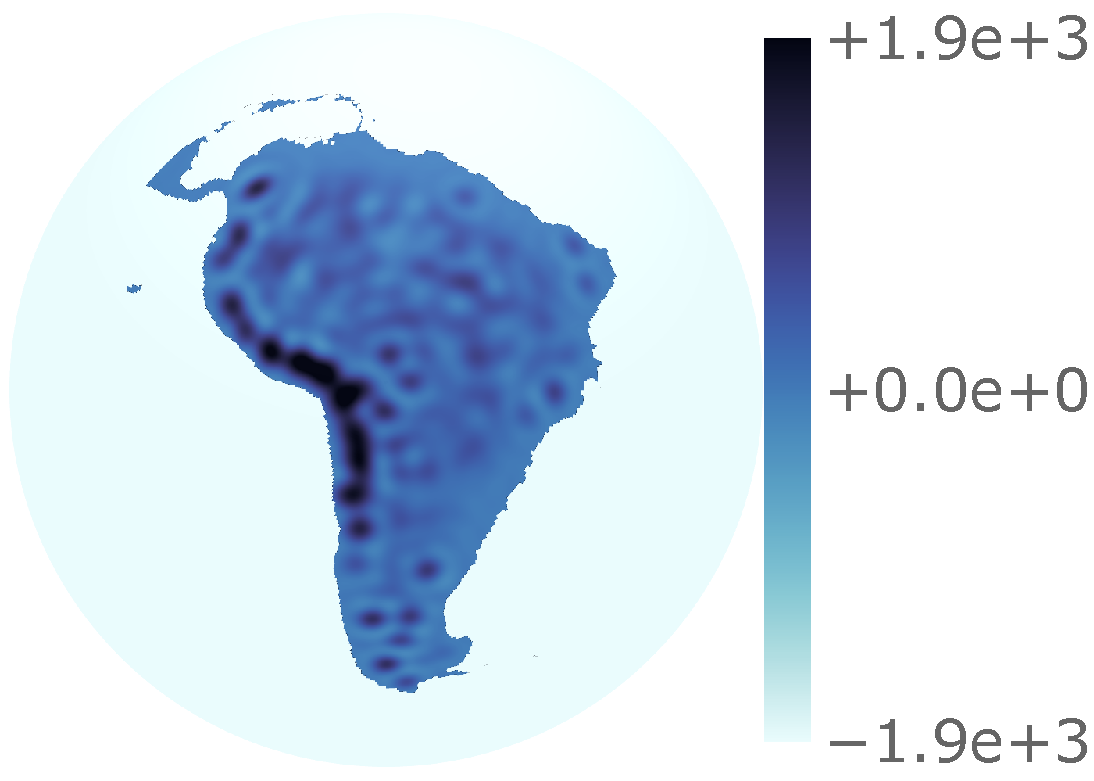
\includegraphics[trim={4 7 3 6},clip,width=.5\textwidth]{slepian_south_america_2smoothed_L128_-10snr_3n_denoised_res512_real.pdf}}
	\hfill
	\subfloat[Denoised \(N_{\sigma}=5\) \newline
		\(\snr{d} = \SI{1.27}{\dB}\)]
	{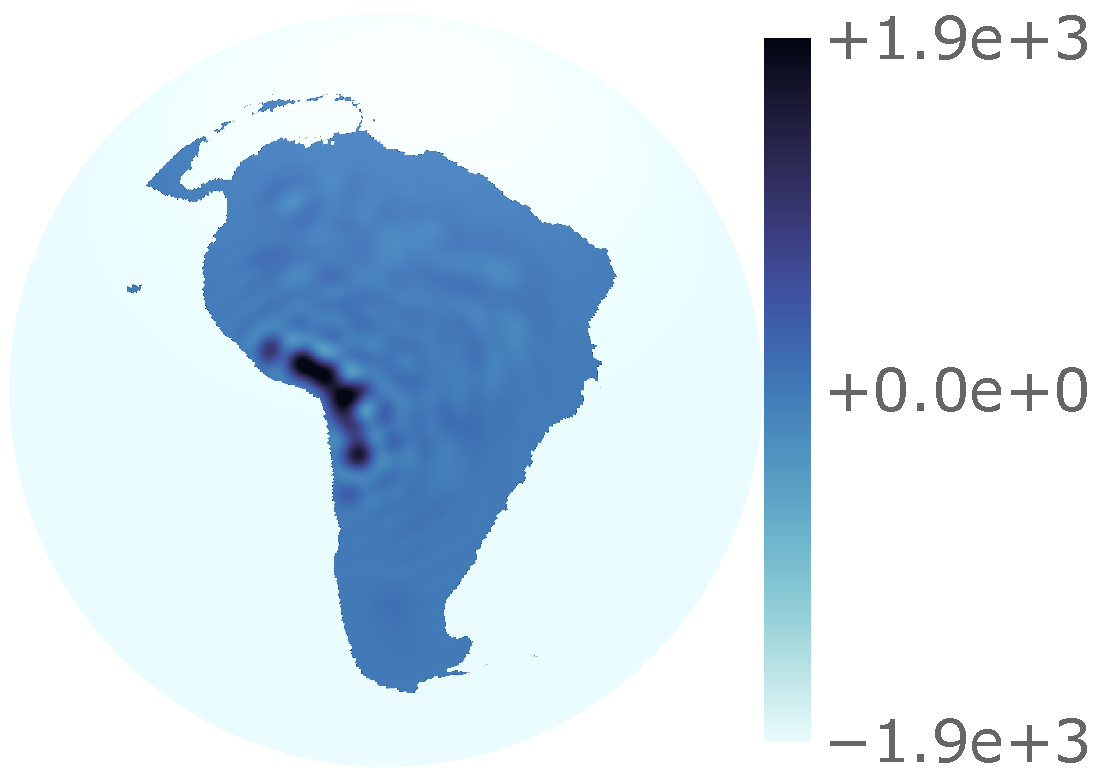
\includegraphics[trim={4 7 3 6},clip,width=.5\textwidth]{slepian_south_america_2smoothed_L128_-10snr_5n_denoised_res512_real.pdf}}
	\caption[
		A denoising demonstration for a map of South America
	]{
		Panel (a) shows the initial noisy signal of the South America region with a signal-to-noise ratio of \(\SI{4.11}{\dB}\).
		The scaling and wavelet coefficients of the noisy signal are calculated and are then hard-thresholded for a few \(N_{\sigma}\) values.
		The corresponding denoised plots for \(N_{\sigma} \in \set{2, 3, 5}\) are shown in panels (b--d). % chktex 8
		At \(N_{\sigma}=2\) the signal-to-noise ratio is boosted by \(\SI{1.56}{\dB}\) to \(\SI{5.67}{\dB}\).
		As more signal is removed the signal-to-noise ratio decreases to \(\SI{4.60}{\dB}\) at \(N_{\sigma}=3\), which is still higher than the initial noisy signal.
		At \(N_{\sigma}=5\) the signal-to-noise ratio is \(\SI{1.27}{\dB}\), where only the Andes remains.
	}\label{fig:chapter4_denoising}
\end{figure}
